\documentclass[%
    debug           = true,
    auto-generate   = true,
    print-ndn       = true,
    plantuml        = true
]{udhbwvst}

\dhbwSetup{%
author          = Simon Eßlinger,
faculty         = Wirtschaft,
field of study  = Wirtschaftsinformatik,
academic year   = 2000,
course          = B,
title           = Eine Arbeit,
subtitle        = Ein Untertitel,
text type       = Projektarbeit 2,
company name    = GitHub,
company logo    = {assets/company-logo.png},
lecturer        = Prof. Dr. Peter Lustig,
location        = Villingen-Schwenningen,
date            = \today,
longest acronym = API,
acronyms        = {%
    \acro{API}{Application Programming Interface}
    \acroplural{API}[API's]{Application Programming Interfaces}
}
}

\begin{document}

\section{This is a section}
\blindtext \dhbwFootcite[Vgl.][42]{example}
\subsection{This is a subsection}
\blindtext \ac{API}
\subsubsection{This is a subsubsection}
\blindtext \acp{API}
\section*{This is a unnumbered section}

\begin{figure}[ht] 
    \centering
    \caption{Example caption}
    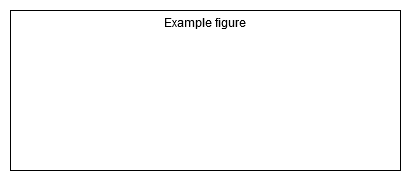
\includegraphics[width=0.7\textwidth]{assets/figure.png} 
    \caption*{\footnotesize{Source: \dhbwCite[69]{example}}}
    \label{fig:goodreference}
\end{figure}

\blindtext

\dhbwFigure{%
    caption = Caption,
    path    = assets/figure.png,
    label   = fig:mytestfig,
    width   = 0.7\textwidth
}

\lipsum

\begin{code}{caption={Express Example},label=lst:lol,language=javascript}{Eigener Code}
const express = require('express')
const app = express()
const port = 3000

app.get('/', (req, res) => res.send('Hello World!'))

app.listen(port, () => console.log(`Example app listening on port ${port}!`))
\end{code}

\blindtext

% \begin{code}{caption={Express Example},label=lst:test,language=javascript}{Eigener Code}
% const express = require('express')
% const app = express()
% const port = 3000

% app.get('/', (req, res) => res.send('Hello World!'))

% app.listen(port, () => console.log(`Example app listening on port ${port}!`))
% \end{code}

\autoref{lst:lol}

\blindtext

\begin{figure}[h]
    \centering
    \caption{Plantuml test}
    \begin{plantuml}
        @startuml

        box "Machine"
            participant "Sensors" as sensors
            participant "OPC UA Server" as opc
        end box
        participant "Cloud" as cloud

        sensors <-> opc
        opc <-> cloud

        @enduml    
    \end{plantuml}
    \caption*{\footnotesize{Quelle: \dhbwCite[69]{example}}}
    \label{fig:plantuml_test}
\end{figure}

\section{lol}

ü ö ä ß test

\lipsum

\begin{dhbwfigure}{caption=Title,label=fig:haha,source={Am Arsch!}}
    \begin{plantuml}
        @startuml
        participant "Cloud" as cloud
        @enduml            
    \end{plantuml}
\end{dhbwfigure}

\autoref{fig:haha}

\end{document}